% \documentclass[a4paper]{article}
% \usepackage[a4paper]{geometry}
\documentclass{article}
\usepackage[body={6.0in,8.5in},top=1in,left=1.25in,nohead]{geometry}
\usepackage{url,verbatim,fancyvrb}
\usepackage{color,gretl}
\usepackage{lucidabr}
\usepackage[authoryear]{natbib}
\usepackage[pdftex]{graphicx}
\usepackage[pdftex,hyperfootnotes=false]{hyperref}
\usepackage[small,bf]{caption}
\usepackage{amsmath}

\definecolor{steel}{rgb}{0.03,0.20,0.45}

\hypersetup{pdftitle={MIDAS in gretl},
            pdfauthor={Allin Cottrell, Jack Lucchetti},
            colorlinks=true,
            linkcolor=blue,
            urlcolor=red,
            citecolor=steel,
            bookmarksnumbered=true,
            plainpages=false
}

\setcounter{secnumdepth}{1}

\begin{document}

\setlength{\parindent}{0pt}
\setlength{\parskip}{1ex}

\title{MIDAS in gretl}
\author{Allin Cottrell, Jack Lucchetti}
%\date{}

\maketitle

These notes describes the state of play with regard to MIDAS (Mixed
Data Sampling---see \citealp{ghysels04}; \citealp{ghysels15};
\citealp{armesto10}) in gretl as of the 2017a release (March
2017). The points covered in these notes are not yet elaborated in the
formal gretl documentation, but the relevant new commands and
functions are described in the current \textit{Gretl Command
  Reference}.

\section{Handling data of more than one frequency}
\label{sec:data-basics}

The essential move in MIDAS is estimation of models including one or
more independent variables observed at a higher frequency than the
dependent variable. Since a gretl dataset formally handles only a
single data frequency it may seem that we have a problem. However, we
have adopted a straightforward solution: a higher frequency series
$x_H$ is represented by a set of $m$ series, each holding the value of
$x_H$ in a sub-period of the ``base'' (lower-frequency) period (where
$m$ is the ratio of the higher frequency to the lower).

This is most easily understood by means of an example. Suppose our
base frequency is quarterly and we wish to include a monthly series in
the analysis. Then a relevant fragment of the gretl dataset might look
as shown in Table~\ref{tab:mdata}. Here, \texttt{gdpc96} is a
quarterly series while \texttt{indpro} is monthly, so $m=12/4=3$ and
the per-month values of \texttt{indpro} are identified by the suffix
\verb|_m|\textit{n}, $n=3,2,1$.

\begin{table}[h]
\small
\begin{verbatim}
                   gdpc96    indpro_m3    indpro_m2    indpro_m1

      1947:1      1934.47      14.3650      14.2811      14.1973
      1947:2      1932.28      14.3091      14.3091      14.2532
      1947:3      1930.31      14.4209      14.3091      14.2253
      1947:4      1960.70      14.8121      14.7562      14.5606
      1948:1      1989.54      14.7563      14.9240      14.8960
      1948:2      2021.85      15.2313      15.0357      14.7842
\end{verbatim}
  \caption{A slice of MIDAS data}
  \label{tab:mdata}
\end{table}

To recover the actual monthly time series for \texttt{indpro} one must
read the three relevant series right-to-left by row. At first glance
this may seem perverse, but in fact it is the most convenient setup
for MIDAS analysis. In such models, the high-frequency variables are
represented by lists of lags, and of course in econometrics it is
standard to give the most recent lag first
$(x_{t-1}, x_{t-2}, \ldots)$.

One can construct such a dataset manually from ``raw'' sources using
hansl's matrix-handling methods or the \texttt{join} command (see
Appendix A for illustrations), but we have added native support for
the common cases shown below.

\begin{center}
\begin{tabular}{ll}
\textit{base frequency} & \textit{higher frequency} \\[4pt]
annual    & quarterly or monthly \\
quarterly & monthly or daily \\
monthly   & daily
\end{tabular}
\end{center}

The examples below mostly pertain to the case of quarterly plus
monthly data. Appendix B has details on our handling of daily data.

The new native methods support creation of a MIDAS-ready dataset in
either of two ways: by selective importation of series from a
database, or by creating two datasets of different frequencies then
merging them.

\subsection{Importation from a database}
\label{sec:db-import}

Here's a simple example, in which we draw from the \texttt{fedstl} (St
Louis Fed) database which is supplied in the gretl distribution:
\begin{code}
clear
open fedstl.bin
data gdpc96
data indpro --compact=spread
store gdp_indpro.gdt
\end{code}

Since \texttt{gdpc96} is a quarterly series, its importation via the
\texttt{data} command establishes a quarterly dataset. Then the
MIDAS work is done by the option \verb|--compact=spread| for the
second invocation of \texttt{data}. This ``spreads'' the series
\texttt{indpro}---which is monthly at source---into three quarterly
series, exactly as shown in Table~\ref{tab:mdata}.

\subsection{Merging two datasets}
\label{sec:data-merge}

In this case we consider an Excel file provided by Eric Ghysels in his
\textsf{MIDAS Matlab Toolbox},\footnote{See
  \url{http://www.unc.edu/~eghysels/} for links.} namely
\texttt{mydata.xlsx}.  This contains quarterly real GDP in Sheet1 and
monthly non-farm payroll employment in Sheet2. A hansl script to build
a MIDAS-style file named \texttt{gdp\_midas.gdt} is shown in
Listing~\ref{lst:ghysels-data}.

\begin{script}[htbp]
  \caption{Building a gretl MIDAS dataset via merger}
  \label{lst:ghysels-data}
\begin{scode}
# sheet 2 contains monthly employment data
open MIDASv2.0/mydata.xlsx --sheet=2
rename VALUE payems
dataset compact 4 spread
# limit to the sample range of the GDP data
smpl 1947:1 2011:2
setinfo payems_m3 --description="Non-farm payroll employment, month 3 of quarter"
setinfo payems_m2 --description="Non-farm payroll employment, month 2 of quarter"
setinfo payems_m1 --description="Non-farm payroll employment, month 1 of quarter"
store payroll_midas.gdt

# sheet 1 contains quarterly GDP data
open MIDASv2.0/mydata.xlsx --sheet=1
rename VALUE qgdp
setinfo qgdp --description="Real quarterly US GDP"
append payroll_midas.gdt
store gdp_midas.gdt
\end{scode}
\end{script}

Note that both series are simply named \texttt{VALUE} in the source
file, so we use gretl's \texttt{rename} command to set distinct and
meaningful names. The heavy lifting is done here by the line
%
\begin{code}
dataset compact 4 spread
\end{code}
%
which tells gretl to compact an entire dataset (in this case, as it
happens, just containing one series) to quarterly frequency using the
``spread'' method. Once this is done, it is straightforward to
\texttt{append} the compacted data to the quarterly GDP dataset.

We will put this dataset to use in subsequent sections. Note that it
is provided in the gretl package (\texttt{gdp\_midas}, which you can
find under the \textsf{Gretl} tab in the practice datafiles window
in the gretl GUI).

\section{The notion of a ``MIDAS list''}
\label{sec:midas-list}

In the following two sections we'll describe functions that (rather
easily) do the right thing if you wish to create lists of lags or
first differences of high-frequency series. However, we should first
be clear about the correct domain for such functions, since they could
produce the most diabolical mash-up of your data if applied to the
wrong sort of list argument---for instance, a regular list containing
distinct series, all observed at the ``base frequency'' of the
dataset.

So let us define a \textbf{MIDAS list}: this is a list of $m$ series
holding per-period values of a \textit{single} high-frequency series,
arranged in the order of most recent first, as illustrated
above. Given the dataset shown in Table~\ref{tab:mdata}, an example
of a correctly formulated MIDAS list would be
%
\begin{code}
list INDPRO = indpro_m3 indpro_m2 indpro_m1
\end{code}
%
Or, since the monthly observations are already in the required order,
we could define the list by means of a ``wildcard'':
%
\begin{code}
list INDPRO = indpro_m*
\end{code}

Having created such a list, one can use the \texttt{setinfo} command
to tell gretl that it's a \textit{bona fide} MIDAS list:
%
\begin{code}
setinfo INDPRO --midas
\end{code}
%
This will spare you some warnings that gretl would otherwise emit when
you call some of the functions described below. This step should not
be necessary, however, if the series in question are the product of a
\texttt{compact} operation with the \texttt{spread} parameter.

\subsection{Inspecting high-frequency data}

The layout of high-frequency data shown in Table~\ref{tab:mdata} is
convenient for running regressions, but not very convenient for
inspecting and checking such data. We therefore provide some methods
for displaying MIDAS data at their ``natural''
frequency. Figure~\ref{fig:data-menu} shows the gretl main window with
the \texttt{gdp\_midas} dataset loaded, along with the menu that pops
up if you right-click with the \texttt{payems} series highlighted.
The items ``Display values'' and ``Time series plot'' show the data
on their original monthly calendar, while the ``Display components''
item shows the three component series on a quarterly calendar, as
in Table~\ref{tab:mdata}.

These methods are also available via the command line. For example,
the commands
%
\begin{code}
list PAYEMS = payems_*
print PAYEMS --byobs --midas
hfplot PAYEMS --with-lines --output=display
\end{code}
%
produce a monthly printout of the payroll employment data, followed by
a monthly time-series plot. (See section~\ref{sec:hfplot} for more on
\texttt{hfplot}.)

\begin{figure}[htbp]
  \centering
  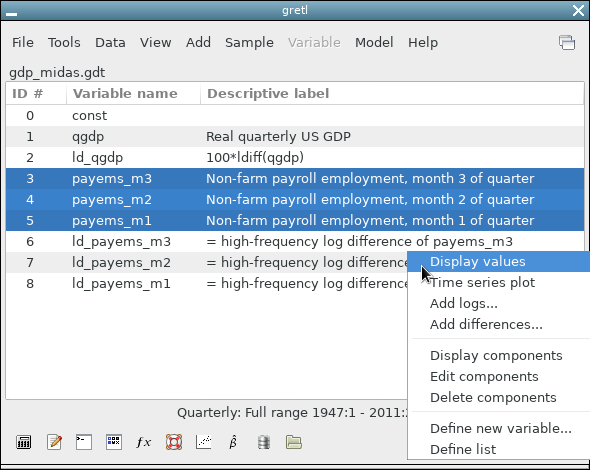
\includegraphics[scale=0.5]{figures/midas-list-menu}
  \caption{MIDAS data menu}
  \label{fig:data-menu}
\end{figure}


\section{High-frequency lag lists}
\label{sec:hflags}

A basic requirement of MIDAS is the creation of lists of
high-frequency lags for use on the right-hand side of a regression
specification. This is possible, but not very convenient, using the
long-standing behavior of gretl's \texttt{lags} function; it is made
easier by a dedicated variant of that function described below.

For illustration we'll consider an example presented in Ghysels'
\textsf{Matlab} implementation of MIDAS: this uses 9 monthly lags of
payroll employment, starting at lag 3, in a model for quarterly GDP.
The estimation period for this model starts in 1985Q1. At this
observation, the stipulation that we start at lag 3 means that the
first (most recent) lag is employment for October 1984,\footnote{That
  is what Ghysels means, but see the sub-section on ``Leads and
  nowcasting'' below for a possible ambiguity in this regard.} and the
9-lag window means that we need to include monthly lags back to
February 1984. Let the per-month employment series be called
\texttt{x\_m3}, \texttt{x\_m2} and \texttt{x\_m1}, and let (quarterly)
lags be represented by \texttt{(-1)}, \texttt{(-2)} and so on. Then
the terms we want are (reading left-to-right by row):
\begin{center}
{\small
\begin{tabular}{ccc}
 . & . & \texttt{x\_m1(-1)} \\
\texttt{x\_m3(-2)} & \texttt{x\_m2(-2)} & \texttt{x\_m1(-2)} \\
\texttt{x\_m3(-3)} & \texttt{x\_m2(-3)} & \texttt{x\_m1(-3)} \\
\texttt{x\_m3(-4)} & \texttt{x\_m2(-4)} & .
\end{tabular}
}
\end{center}

We could construct such a list in gretl using the following
standard syntax. (Note that the third argument of 1 to
\texttt{lags} below tells gretl that we want the terms ordered ``by
lag'' rather than ``by variable''; this is required to respect the
order of the terms shown above.)
\begin{code}
list X = x_m*
# create lags for 4 quarters, "by lag"
list XL = lags(4,X,1)
# convert the list to a matrix
matrix tmp = XL
# trim off the first two elements, and the last
tmp = tmp[3:11]
# and convert back to a list
XL = tmp
\end{code}

However, the following specialized syntax is more convenient:
\begin{code}
list X = x_m*
setinfo X --midas
# create high-frequency lags 3 to 11
list XL = hflags(3, 11, X)
\end{code}

In the case of \texttt{hflags} the length of the list given as the
third argument defines the ``compaction ratio'' ($m=3$ in this
example); we can (in fact, must) specify the lags we want in
high-frequency terms; and ordering of the generated series by lag is
automatic. 

Word to the wise: do not use \texttt{hflags} on anything other than a
\textbf{MIDAS list} as defined in section~\ref{sec:midas-list}, unless
perhaps you have some special project in mind and really know what you
are doing.

\subsection{Leads and nowcasting}

Before leaving the topic of lags, it is worth commenting on the
question of leads and so-called ``nowcasting''---that is, prediction
of the current value of a lower-frequency variable before its
measurement becomes available.

In a regular dataset where all series are of the same frequency,
lag 1 means the observation from the previous period, lag 0 is
equivalent to the current observation, and lag $-1$ (or lead 1) is the
observation for the next period into the relative future.

When considering high-frequency lags in the MIDAS context, however,
there is no uniquely determined high-frequency sub-period which is
temporally coincident with a given low-frequency period. The placement
of high-frequency lag 0 therefore has to be a matter of
convention. Unfortunately, there are two incompatible conventions in
currently available MIDAS software, as follows.
%
\begin{itemize}
\item High-frequency lag 0 corresponds to the \textit{first}
  sub-period within the current low-frequency period. This is what we
  find in Eric Ghysels' \textsf{MIDAS Matlab Toolbox}; it's also
  clearly stated and explained in \cite{armesto10}.
\item High-frequency lag 0 corresponds to the \textit{last} sub-period
  in the current low-frequency period. This convention is employed in
  the \texttt{midasr} package for \textsf{R}.\footnote{See
    \url{http://cran.r-project.org/web/packages/midasr/}, and for
    documentation
    \url{https://github.com/mpiktas/midasr-user-guide/raw/master/midasr-user-guide.pdf}.}
\end{itemize}
%
Consider, for example, the quarterly/monthly case. In \textsf{Matlab},
high-frequency (HF) lag 0 is the first month of the current quarter,
HF lag 1 is the last month of the prior quarter, and so on. In
\texttt{midasr}, however, HF lag 0 is the last month of the current
quarter, HF lag 1 the middle month of the quarter, and HF lag 3
is the first one to take you ``back in time'' relative to the start
of the current quarter, namely to the last month of the prior
quarter.

In gretl we have chosen to employ the first of these conventions. So
Lag 1 points to the most recent sub-period in the previous
base-frequency period, lag 0 points to the first sub-period in the
current period, and lag $-1$ to the second sub-period within the
current period. Continuing with the quarterly/monthly case, monthly
observations for lags 0 and $-1$ are likely to become available before
a measurement for the quarterly variable is published (possibly also a
monthly value for lag $-2$). The first ``truly future'' lead does not
occur until lag $-3$.

The \texttt{hflags} function supports negative lags. Suppose one
wanted to use 9 lags of a high-frequency variable,
$-1, 0, 1,\ldots, 7$, for nowcasting. Given a suitable MIDAS list,
\texttt{X}, the following would do the job:
\begin{code}
list XLnow = hflags(-1, 7, X)
\end{code}

This means that one could generate a forecast for the current
low-frequency period (which is not yet completed and for which no
observation is available) using data from two sub-periods into the
low-frequency period (e.g.\ the first two months of the quarter).

\section{High-frequency first differences}

When working with non-stationary data one may wish to take first
differences, and in the MIDAS context that probably means
high-frequency differences of the high-frequency data. Note that the
ordinary gretl functions \texttt{diff} and \texttt{ldiff} will
\textit{not} do what is wanted for series such as \texttt{indpro}, as
shown in Table~\ref{tab:mdata}: these functions will give per-month
\textit{quarterly} differences of the data (month 3 of the current
quarter minus month 3 of the previous quarter, and so on).

To get the desired result one could create the differences before
compacting the high-frequency data but this may not be convenient, and
it's not compatible with the method of constructing a MIDAS dataset
shown in section~\ref{sec:db-import}. The alternative is to employ the
specialized differencing function \texttt{hfdiff}. This takes one
required argument, a \textbf{MIDAS list} as defined in
section~\ref{sec:midas-list}. A second, optional argument is a scalar
multiplier (with default value 1.0); this permits scaling the output
series by a constant. There's also an \texttt{hfldiff} function for
creating high-frequency log differences; this has the same syntax as
\texttt{hfdiff}.

So for example, the following creates a list of high-frequency
percentage changes (100 times log-difference) then a list of
high-frequency lags of the changes.
%
\begin{code}
list X = indpro_*
setinfo X --midas
list dX = hfldiff(X, 100)
list dXL = hflags(3, 11, dX)
\end{code}

If you only need the series in the list \texttt{dXL}, however, you can
nest these two function calls:
%
\begin{code}
list dXL = hflags(3, 11, hfldiff(X, 100))
\end{code}

\section{Parsimonious parameterizations}
\label{sec:hparams}

The simplest MIDAS regression specification---known as ``unrestricted
MIDAS'' or U-MIDAS---simply includes $p$ lags of a high-frequency
regressor, each with its own parameter to be estimated (which can be
done via OLS). It is more common, however, to enforce parsimony by
making the individual coefficients on lagged high-frequency terms a
function of a relatively small number of hyperparameters. This
presents a couple of computational questions: how to calculate the
per-lag coefficients given the values of the hyperparameters, and how
best to estimate the value of the hyperparameters?

Hansl is functional enough to allow a savvy user to address these
questions from scratch, but of course it's helpful to have some
built-in high-level functionality. At present gretl can handle
natively four commonly used parameterizations: normalized exponential
Almon, normalized beta (with or without a zero last coefficient) and
plain (non-normalized) Almon polynomial. The Almon variants take one
or more parameters (two being a common choice), and the beta takes
either two or three parameters.\footnote{Two is the standard case; see
  Appendix C for details.}  All are handled by the functions
\texttt{mweights} and \texttt{mgradient}. These functions work as
follows.
\begin{itemize}
\item \texttt{mweights} takes three arguments: the number of lags
  required ($p$), the $k$-vector of hyperparameters ($\theta$), and an
  integer code or string indicating the method (see
  Table~\ref{tab:midas-parm}). It returns a $p$-vector containing the
  coefficients.
\item \texttt{mgradient} takes three arguments, just like
  \texttt{mweights}. However, this function returns a $p \times k$
  matrix holding the (analytical) gradient of the $p$ coefficients or
  weights with respect to the $k$ elements of $\theta$.
\end{itemize}

\begin{table}[htbp]
  \centering
  \begin{tabular}{lcl}
    \textit{Parameterization} & 
      \textit{code} & \textit{string} \\[4pt]
    Normalized exponential Almon & 1 & \verb|"nealmon"| \\
    Normalized beta, zero last lag & 2 & \verb|"beta0"| \\
    Normalized beta, non-zero last lag & 3 & \verb|"betan"| \\
    Almon polynomial & 4 & \verb|"almonp"| \\
  \end{tabular}
  \caption{MIDAS parameterizations}
  \label{tab:midas-parm}
\end{table}

An additional function is provided for convenience: it is named
\texttt{mlincomb} and it combines \texttt{mweights} with the
long-standing \texttt{lincomb} function, which takes a list (of
series) argument followed by a vector of coefficients and produces a
series result, namely a linear combination of the elements of the
list. If we have a suitable list \texttt{L} available, we can
do, for example,
\begin{code}
series foo = mlincomb(L, theta, "beta0")
\end{code}
This is equivalent to
\begin{code}
series foo = lincomb(L, mweights(nelem(L), theta, "beta0"))
\end{code}
but saves a little typing and some CPU cycles.

\section{Estimating MIDAS models}
\label{sec:estimation}

Gretl offers a dedicated command, \texttt{midasreg}, for estimation of
MIDAS models. (There's a corresponding item, \textsf{MIDAS}, under the
\textsf{Time series} section of the \textsf{Model} menu in the gretl
GUI.) We begin by discussing that, then move on to possibilities for
defining your own estimator.

The syntax of \texttt{midasreg} looks like this:

\texttt{midasreg \textsl{depvar} \textsl{xlist} ;
\textsl{midas-terms} [ \textsl{options} ]}

The \texttt{\textsl{depvar}} slot takes the name (or series ID number)
of the dependent variable, and \texttt{\textsl{xlist}} is the list of
regressors that are observed at the same frequency as the dependent
variable; this list may contain lags of the dependent variable. The
\texttt{\textsl{midas-terms}} slot accepts one or more specification(s)
for high-frequency terms. Each of these specifications must conform to
one or other of the following patterns:

\begin{tabular}{ll}
1 & \texttt{mds(\textsl{mlist}, \textsl{minlag}, 
   \textsl{maxlag}, \textsl{type}, \textsl{theta})} \\
2 & \texttt{mdsl(\textsl{llist}, \textsl{type}, \textsl{theta})}
\end{tabular}

In case 1 \texttt{\textsl{mlist}} must be a \textbf{MIDAS list}, as
defined above, which contains a full set of per-period series (but no
lags). Lags will be generated automatically, governed by the
\texttt{\textsl{minlag}} and \texttt{\textsl{maxlag}} (integer)
arguments, which may be given as numerical values or the names of
predefined scalar variables. The integer (or string)
\texttt{\textsl{type}} argument represents the type of
parameterization; in addition to the values 1 to 4 defined in
Table~\ref{tab:midas-parm} a value of 0 (or the string
\verb|"umidas"|) indicates unrestricted MIDAS.

In case 2 \texttt{\textsl{llist}} is assumed to be a list that
already contains the required set of high-frequency lags---as may be
obtained via the \texttt{hflags} function described in
section~\ref{sec:hflags}---hence \texttt{\textsl{minlag}} and
\texttt{\textsl{maxlag}} are not wanted.

The final \texttt{\textsl{theta}} argument is optional in most cases
(implying an automatic initialization of the hyperparameters). If this
argument is given it must take one of the following forms:
\begin{enumerate}
\item The name of a matrix (vector) holding initial values for the
  hyperparameters, or a simple expression which defines a matrix
  using scalars, such as \texttt{\{1, 5\}}.
\item The keyword \texttt{null}, indicating that an automatic
  initialization should be used (as happens when this argument is
  omitted).
\item An integer value (in numerical form), indicating how many
  hyperparameters should be used (which again calls for
  automatic initialization).
\end{enumerate}
The third of these forms is required if you want automatic
initialization in the Almon polynomial case, since we need to know how
many terms you wish to include. (In the normalized exponential Almon
case we default to the usual two hyperparameters if
\texttt{\textsl{theta}} is omitted or given as \texttt{null}.)

The \texttt{midasreg} syntax allows the user to specify multiple
high-frequency predictors, if wanted: these can have different lag
specifications, different parameterizations and/or different
frequencies.

The options accepted by \texttt{midasreg} include \option{quiet}
(suppress printed output), \option{verbose} (show detail of
iterations, if applicable) and \option{robust} (use a HAC estimator of
the Newey--West type in computing standard errors).  Two additional
specialized options are described below.

\subsection{Examples of usage}

Suppose we have a dependent variable named \texttt{dy} and a MIDAS
list named \texttt{dX}, and we wish to run a MIDAS regression using
one lag of the dependent variable and high-frequency lags 1 to 10 of
the series in \texttt{dX}. The following will produce U-MIDAS
estimates:
%
\begin{code}
midasreg dy const dy(-1) ; mds(dX, 1, 10, 0)
\end{code}
%
The next lines will produce estimates for the normalized exponential
Almon parameterization with two coefficients, both initialized to
zero:
%
\begin{code}
midasreg dy const dy(-1) ; mds(dX, 1, 10, "nealmon", {0,0})
\end{code}
%
In the examples above, the required lags will be added to the dataset
automatically then deleted after use. If you are estimating several
models using a single set of MIDAS lags it is more efficient to create
the lags once and use the \texttt{mdsl} specifier.  For example, the
following estimates three variant parameterizations (exponential
Almon, beta with zero last lag, and beta with non-zero last lag) on
the same data:
\begin{code}
list dXL = hflags(1, 10, dX)
midasreg dy 0 dy(-1) ; mdsl(dXL, "nealmon", {0,0})
midasreg dy 0 dy(-1) ; mdsl(dXL, "beta0", {1,5})
midasreg dy 0 dy(-1) ; mdsl(dXL, "betan", {1,1,0})
\end{code}

Any additional MIDAS terms should be separated by spaces, as in
\begin{code}
midasreg dy const dy(-1) ; mds(dX,1,9,1,theta1) mds(Z,1,6,3,theta2)
\end{code}

\subsection{Replication exercise}

We give a substantive illustration of \texttt{midasreg} in
Listing~\ref{lst:midasreg-ghysels}. This replicates the first
practical example discussed by Ghysels in the user's guide titled
\textit{MIDAS Matlab Toolbox},\footnote{See \cite{ghysels15}. This
  document announces itself as Version 2.0 of the guide and is dated
  November 1, 2015. The example we're looking at appears on pages
  24--26; the associated \textsf{Matlab} code can be found in the
  program \texttt{appADLMIDAS1.m}.}
The dependent variable is the quarterly log-difference of
real GDP, named \texttt{dy} in our script. The independent variables
are the first lag of \texttt{dy} and monthly lags 3 to 11 of the
monthly log-difference of non-farm payroll employment (named
\texttt{dXL} in our script). Formally, the model may be written
as
\[
  y_t = \alpha + \beta y_{t-1} + \gamma W(x_{\tau-3}, x_{\tau-4},\dots,
  x_{\tau-11}; \theta) + \varepsilon_t
\]
where $W(\cdot)$ is the weighting function associated with a given
MIDAS specification, $\theta$ is a vector of hyperparameters, and
$\tau$ represents ``high-frequency time.'' In the case of the
non-normalized Almon polynomial the $\gamma$ coefficient is
identically 1.0 and is omitted; and in the U-MIDAS case the model
comes down to
\[
  y_t = \alpha + \beta y_{t-1} + \sum_{i=1}^9 \delta_i x_{\tau-i-2}
  + \varepsilon_t
\]

The script exercises all five of the parameterizations mentioned
above,\footnote{The \textsf{Matlab} program includes an additional
  parameterization not supported by gretl, namely a step-function.}
and in each case the results of 9 pseudo-out-of-sample forecasts are
recorded so that their Root Mean Square Errors can be compared.

\begin{script}[p]
  \caption{Script to replicate results given by Ghysels}
  \label{lst:midasreg-ghysels}
\begin{scode}
set verbose off
open gdp_midas.gdt --quiet

# form the dependent variable
series dy = 100 * ldiff(qgdp)
# form list of high-frequency lagged log differences
list X = payems*
list dXL = hflags(3, 11, hfldiff(X, 100))
# initialize matrix to collect forecasts
matrix FC = {}

# estimation sample
smpl 1985:1 2009:1

print "=== unrestricted MIDAS (umidas) ==="
midasreg dy 0 dy(-1) ; mdsl(dXL, 0)
fcast --out-of-sample --static --quiet
FC ~= $fcast

print "=== normalized beta with zero last lag (beta0) ==="
midasreg dy 0 dy(-1) ; mdsl(dXL, 2, {1,5})
fcast --out-of-sample --static --quiet
FC ~= $fcast

print "=== normalized beta, non-zero last lag (betan) ==="
midasreg dy 0 dy(-1) ; mdsl(dXL, 3, {1,1,0})
fcast --out-of-sample --static --quiet
FC ~= $fcast

print "=== normalized exponential Almon (nealmon) ==="
midasreg dy 0 dy(-1) ; mdsl(dXL, 1, {0,0})
fcast --out-of-sample --static --quiet
FC ~= $fcast

print "=== Almon polynomial (almonp) ==="
midasreg dy 0 dy(-1) ; mdsl(dXL, 4, 4)
fcast --out-of-sample --static --quiet
FC ~= $fcast

smpl 2009:2 2011:2
matrix my = {dy}
print "Forecast RMSEs:"
printf "  umidas  %.4f\n", fcstats(my, FC[,1])[2]
printf "  beta0   %.4f\n", fcstats(my, FC[,2])[2]
printf "  betan   %.4f\n", fcstats(my, FC[,3])[2]
printf "  nealmon %.4f\n", fcstats(my, FC[,4])[2]
printf "  almonp  %.4f\n", fcstats(my, FC[,5])[2]
\end{scode}
\end{script}

\begin{script}[p]
  \caption{Replication of Ghysels' results, partial output}
  \label{ghysels-out}
\begin{scode}
=== normalized beta, non-zero last lag (betan) ===
Model 3: MIDAS (NLS), using observations 1985:1-2009:1 (T = 97)
Using L-BFGS-B with conditional OLS
Dependent variable: dy

              estimate    std. error   t-ratio   p-value 
  -------------------------------------------------------
  const       0.748578    0.146404      5.113    1.74e-06 ***
  dy_1        0.248055    0.118903      2.086    0.0398   **

        MIDAS list dXL, high-frequency lags 3 to 11
   
  HF_slope    1.72167     0.582076      2.958    0.0039   ***
  Beta1       0.998501    0.0269479    37.05     1.10e-56 ***
  Beta2       2.95148     2.93404       1.006    0.3171  
  Beta3      -0.0743143   0.0271273    -2.739    0.0074   ***

Sum squared resid    28.78262   S.E. of regression   0.562399
R-squared            0.356376   Adjusted R-squared   0.321012
Log-likelihood      -78.71248   Akaike criterion     169.4250
Schwarz criterion    184.8732   Hannan-Quinn         175.6715

=== Almon polynomial (almonp) ===
Model 5: MIDAS (NLS), using observations 1985:1-2009:1 (T = 97)
Using Levenberg-Marquardt algorithm
Dependent variable: dy

              estimate    std. error   t-ratio   p-value 
  -------------------------------------------------------
  const       0.741403    0.146433      5.063    2.14e-06 ***
  dy_1        0.255099    0.119139      2.141    0.0349   **

        MIDAS list dXL, high-frequency lags 3 to 11

  Almon0      1.06035     1.53491       0.6908   0.4914  
  Almon1      0.193615    1.30812       0.1480   0.8827  
  Almon2     -0.140466    0.299446     -0.4691   0.6401  
  Almon3      0.0116034   0.0198686     0.5840   0.5607  

Sum squared resid    28.66623   S.E. of regression   0.561261
R-squared            0.358979   Adjusted R-squared   0.323758
Log-likelihood      -78.51596   Akaike criterion     169.0319
Schwarz criterion    184.4802   Hannan-Quinn         175.2784

Forecast RMSEs:
  umidas  0.5424
  beta0   0.5650
  betan   0.5210
  nealmon 0.5642
  almonp  0.5329
\end{scode}
\end{script}

The data file used in the replication, \texttt{gdp\_midas.gdt}, was
contructed as described in section~\ref{sec:data-merge} (and as noted
there, it is included in the current gretl package). Part of the
output from the replication script is shown in
Listing~\ref{ghysels-out}. The $\gamma$ coefficient is labeled
\texttt{HF\_slope} in the gretl output.

For reference, output from \textsf{Matlab} (version R2016a for Linux)
is available at
\url{http://gretl.sourceforge.net/midas/matlab_output.txt}. For the
most part (in respect of regression coefficients and auxiliary
statistics such as $R^2$ and forecast RMSEs), gretl's output agrees
with that of \textsf{Matlab} to the extent that one can reasonably
expect on nonlinear problems---that is, to at least 4 significant
digits in all but a few instances.\footnote{Nonlinear results, even
  for a given software package, are subject to slight variation
  depending on the compiler used and the exact versions of supporting
  numerical libraries.}  Standard errors are not quite so close across
the two programs, particularly for the hyperparameters of the beta and
exponential Almon functions. We show these in Table~\ref{tab:stderrs}.

\begin{table}[hbtp]
  \centering
  \begin{tabular}{rcccccc}
 & \multicolumn{2}{c}{2-param beta \qquad} & 
  \multicolumn{2}{c}{3-param beta \qquad} &
  \multicolumn{2}{c}{Exp Almon \qquad} \\[4pt]
 & \textsf{Matlab} & \textsf{gretl} & 
   \textsf{Matlab} & \textsf{gretl} &
   \textsf{Matlab} & \textsf{gretl} \\
const    & 0.135 & 0.140 & 0.143 & 0.146 & 0.135 & 0.140 \\
dy(-1)   & 0.116 & 0.118 & 0.116 & 0.119 & 0.116 & 0.119 \\
HF slope & 0.559 & 0.575 & 0.566 & 0.582 & 0.562 & 0.575 \\
$\theta_1$ & 0.067 & 0.106 & 0.022 & 0.027 & 2.695 & 6.263 \\
$\theta_2$ & 9.662 & 17.140 & 1.884 & 2.934 & 0.586 & 1.655 \\
$\theta_3$ &        &	     & 0.022 & 0.027 \\
\end{tabular}
  \caption{Comparison of standard errors from MIDAS regressions}
  \label{tab:stderrs}
\end{table}

Differences of this order are not unexpected, however, when different
methods are used to calculate the covariance matrix for a nonlinear
regression. The \textsf{Matlab} standard errors are based on a
numerical approximation to the Hessian at convergence, while those
produced by gretl are based on a Gauss--Newton Regression, as
discussed and recommended in \citet[chapter 6]{davidson-mackinnon04}.

\subsection{Underlying methods}

The \texttt{midasreg} command calls one of several possible estimation
methods in the background, depending on the MIDAS specification(s). As
shown in Listing~\ref{ghysels-out}, this is flagged in a line of
output immediately preceding the ``\texttt{Dependent variable}'' line.
If the only specification type is U-MIDAS, the method is
OLS. Otherwise it is one of three variants of Nonlinear Least Squares.
\begin{itemize}
\item Levenberg--Marquardt. This is the back-end for gretl's
  \texttt{nls} command.
\item L-BFGS-B with conditional OLS. L-BFGS is a ``limited memory''
  version of the BFGS optimizer and the trailing ``-B'' means that it
  supports bounds on the parameters, which is useful for reasons given
  below.
\item Golden Section search with conditional OLS. This is a line
  search method, used only when there is a just a single
  hyperparameter to estimate.
\end{itemize}

Levenberg--Marquardt is the default NLS method, but if the MIDAS
specifications include any of the beta variants or normalized
exponential Almon we switch to L-BFGS-B, \textit{unless} the user
gives the \option{levenberg} option. The ability to set bounds on the
hyperparameters via L-BFGS-B is helpful, first because the beta
parameters (other than the third one, if applicable) must be
non-negative but also because one is liable to run into numerical
problems (in calculating the weights and/or gradient) if their values
become too extreme. For example, we have found it useful to place
bounds of $-2$ and $+2$ on the exponential Almon parameters.

Here's what we mean by ``conditional OLS'' in the context of L-BFGS-B
and line search: the search algorithm itself is only responsible for
optimizing the MIDAS hyperparameters, and when the algorithm calls for
calculation of the sum of squared residuals given a certain
hyperparameter vector we optimize the remaining parameters
(coefficients on base-frequency regressors, slopes with respect to
MIDAS terms) via OLS.


\subsection{Other specialized options}

We mentioned above the standard options that are supported by the
\texttt{midasreg} command, plus the \option{levenberg} option; here we
explain two additional options, \option{clamp-beta} and
\option{breaktest}.

First, a case can be made for a variant of the normalized beta
parameterization that is even more parsimonious than those discussed
above: we take as a basis the two-parameter case (which implies a zero
coefficient on the last lag) and ``clamp'' the first parameter,
$\theta_1$, at 1.0; the second parameter is then optimized, subject to
the constraint $\theta_2 \ge 1.0$. This variant allows for a wide
range of patterns of declining weights while arguably avoiding
over-fitting of the weighting function to the estimation sample.
Although it is bound to fit somewhat less well than the more general
beta specifications in-sample it may be more effective in
out-of-sample forecasting \citep{ghysels-qian16}. This is supported
under \texttt{midasreg} as follows: you specify the two-parameter beta
option (\textsl{type} = 2, see section~\ref{sec:hparams}) but add the
option flag \option{clamp-beta}. At present this option is valid only
if the regression contains a single MIDAS specification.

Second, the \option{breaktest} option can be used to carry out the
Quandt Likelihood Ratio (QLR) test for a structural break at the stage
of running the final Gauss--Newton regression (to check for
convergence and calculate the covariance matrix of the parameter
estimates).  This can be a useful aid to diagnosis, since
non-homogeneity of the data over the estimation period can lead to
numerical problems in nonlinear estimation, besides compromising the
forecasting capacity of the resulting equation. For example, when this
option is given with the command to estimate the ``\texttt{BetaNZ}''
model shown in Listing~\ref{ghysels-out}, the following result is
appended to the standard output:
%
\begin{code}
QLR test for structural break -
  Null hypothesis: no structural break
  Test statistic: chi-square(6) = 35.1745 at observation 2005:2
  with asymptotic p-value = 0.000127727
\end{code}
%
Despite the strong evidence for a structural break, in this case the
nonlinear estimator appears to converge successfully, but one might
wonder if a shorter estimation period could provide better
out-of-sample forecasts.

\subsection{Defining your own MIDAS estimator}

As explained above, the \texttt{midasreg} command is in effect a
``wrapper'' for various underlying methods. Some users may wish to
undo the wrapping. (This would be required if you wish to introduce
any nonlinearity other than that associated with the stock MIDAS
parameterizations, or to define your own MIDAS parameterization).

Anyone with ambitions in this direction will presumably be quite
familiar with the commands and functions available in hansl, gretl's
scripting language, so we will not say much here beyond presenting a
couple of examples. First we show how the \texttt{nls} command can be
used, along with the MIDAS-related functions described in
section~\ref{sec:hparams}, to estimate a model with the exponential
Almon specification.
%
\begin{code}
open gdp_midas.gdt --quiet
series dy = 100 * ldiff(qgdp)
series dy1 = dy(-1)
list X = payems*
list dXL = hflags(3, 11, hfldiff(X, 100))

smpl 1985:1 2009:1

# initialization via OLS
series mdX = mean(dXL)
ols dy 0 dy1 mdX --quiet
matrix b = $coeff | {0,0}'
scalar p = nelem(dXL)

# convenience matrix for computing gradient
matrix mdXL = {dXL}

# normalized exponential Almon via nls
nls dy = b[1] + b[2]*dy1 + b[3]*mdx
  series mdx = mlincomb(dXL, b[4:], 1)
  matrix grad = mgradient(p, b[4:], 1)
  deriv b = {const, dy1, mdx} ~ (b[3] * mdXL * grad)
  param_names "const dy(-1) HF_slope Almon1 Almon2"
end nls
\end{code}

Listing~\ref{lst:manual-beta1} presents a more ambitious example: we
use \texttt{GSSmin} (Golden Section minimizer) to estimate a MIDAS
model with the ``one-parameter beta'' specification (that is, the
two-parameter beta with $\theta_1$ clamped at 1). Note that while the
function named \texttt{beta1\_SSR} is specialized to the given
parameterization, \texttt{midas\_GNR} is a fairly general means of
calculating the Gauss--Newton regression for an ADL(1) MIDAS
model, and it could be generalized further without much difficulty.

\begin{script}[p]
  \caption{Manual MIDAS: one-parameter beta specification}
  \label{lst:manual-beta1}
\begin{scode}
set verbose off

function scalar beta1_SSR (scalar th2, const series y,
                           const series x, list L)
  matrix theta = {1, th2}
  series mdx = mlincomb(L, theta, 2)
  # run OLS conditional on theta
  ols y 0 x mdx --quiet
  return $ess
end function

function matrix midas_GNR (const matrix theta, const series y,
                           const series x, list L, int type)
  # Gauss-Newton regression
  series mdx = mlincomb(L, theta, type)
  ols y 0 x mdx --quiet
  matrix b = $coeff
  matrix u = {$uhat}
  matrix mgrad = mgradient(nelem(L), theta, type)
  matrix M = {const, x, mdx} ~ (b[3] * {L} * mgrad)
  matrix V
  set svd on # in case of strong collinearity
  mols(u, M, null, &V)
  return (b | theta) ~ sqrt(diag(V))
end function

/* main */

open gdp_midas.gdt --quiet

series dy = 100 * ldiff(qgdp)
series dy1 = dy(-1)
list dX = ld_payem*
list dXL = hflags(3, 11, dX)

# estimation sample
smpl 1985:1 2009:1

matrix b = {0, 1.01, 100}
# use Golden Section minimizer
SSR = GSSmin(b, beta1_SSR(b[1], dy, dy1, dXL), 1.0e-6)
printf "SSR (GSS) = %.15g\n", SSR
matrix theta = {1, b[1]}' # column vector needed
matrix bse = midas_GNR(theta, dy, dy1, dXL, 2)
bse[4,2] = $nan # mask std error of clamped coefficient
modprint bse "const dy(-1) HF_slope Beta1 Beta2"
\end{scode}
\end{script}


\section{MIDAS-related plots}
\label{sec:hfplot}

In the context of MIDAS analysis one may wish to produce time-series
plots which show high- and low-frequency data in correct registration
(as in Figures 1 and 2 in \citealp{armesto10}).  This can be done using
the \texttt{hfplot} command, which has the following syntax:

\texttt{hfplot} \textsl{midas-list} \texttt{[; }\textsl{lflist} 
\texttt{]} \textsl{options}

The required argument is a MIDAS list, as defined above. Optionally,
one or more lower-frequency series (\textsl{lflist}) can be added to
the plot following a semicolon. Supported options are
\option{with-lines}, \option{time-series} and \option{output}. These
have the same effects as with the gretl's \texttt{gnuplot} command.

An example based on Figure 1 in \cite{armesto10} is shown in
Listing~\ref{lst:armesto} and Figure~\ref{fig:armesto}.

\begin{script}[p]
  \caption{Replication of a plot from Armesto et al}
  \label{lst:armesto}
\begin{scode}
open gdp_midas.gdt

# form and label the dependent variable
series dy = log(qgdp/qgdp(-1))*400
setinfo dy --graph-name="GDP"

# form list of annualized HF differences
list X = payems*
list dX = hfldiff(X, 1200)
setinfo dX --graph-name="Payroll Employment"

smpl 1980:1 2009:1
hfplot dX ; dy --with-lines --time-series --output=display
\end{scode}
\end{script}

\begin{figure}[p]
  \centering
  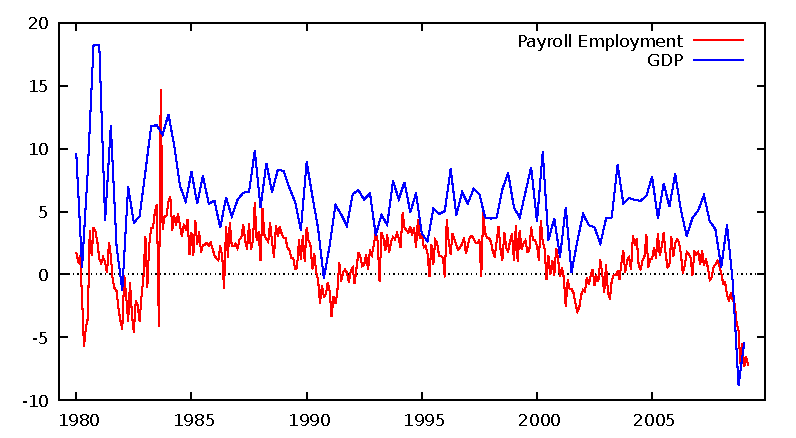
\includegraphics{figures/armesto_plot}
  \caption{Quarterly GDP and monthly Payroll Employment,
  annualized percentage changes}
  \label{fig:armesto}
\end{figure}

Another sort of plot which may be useful shows the ``gross''
coefficients on the lags of the high-frequency series in a MIDAS
regression---that is, the normalized weights multiplied by the
\texttt{HF\_slope} coefficient. After estimation of a MIDAS model in
the gretl GUI this is available via the item \textsf{MIDAS
  coefficients} under the \textsf{Graphs} menu in the model window. It
is also easily generated via script, since the \dollar{model} bundle
that becomes available following the \texttt{midasreg} command
contains a matrix, \texttt{midas\_coeffs}, holding these
coefficients. So the following is sufficient to display the plot:
%
\begin{code}
matrix m = $model.midas_coeffs
gnuplot --matrix=m --with-lp --fit=none --output=display \
  { set title "MIDAS coefficients"; set ylabel ''; }
\end{code}

Caveat: this feature is at present available only for models with a
single MIDAS specification.

\bibliographystyle{gretl}
\bibliography{gretl}

\appendix

\clearpage

\section*{Appendix A: alternative MIDAS data methods}
\label{app:data-methods}

\subsection*{Importation via a column vector}

Listing~\ref{hflist} illustrates how one can construct via hansl a
``midas list'' from a matrix (column vector) holding data of a higher
frequency than the given dataset. In practice one would probably read
high frequency data from file using the \texttt{mread} function, but
here we just construct an artificial sequential vector.

Note the check in the \texttt{high\_freq\_list} function: we determine
the current sample size, \texttt{T}, and insist that the input matrix
is suitably dimensioned, with a single column of length equal to
\texttt{T} times the compaction factor (here 3, for monthly to
quarterly).

\begin{script}[htbp]
  \caption{Create a midas list from a matrix}
  \label{hflist}
\begin{scode}
function list high_freq_list (const matrix x, int compfac, string vname)
  list ret = null
  scalar T = $nobs
  if rows(x) != compfac*T || cols(x) != 1
     funcerr "Invalid x matrix"
  endif
  matrix m = mreverse(mshape(x, compfac, T))'
  loop i=1..compfac --quiet
    scalar k = compfac + 1 - i
    ret += genseries(sprintf("%s%d", vname, k), m[,i])
  endloop
  setinfo ret --midas 
  return ret
end function

# construct a little "quarterly" dataset
nulldata 12
setobs 4 1980:1

# generate "monthly" data, 1,2,...,36
matrix x = seq(1,3*$nobs)'
print x
# turn into midas list
list H = high_freq_list(x, 3, "test_m")
print H --byobs
\end{scode}
\end{script}

The final command in the script should produce

{
\small
\begin{verbatim}
            test_m3      test_m2      test_m1

1980:1            3            2            1
1980:2            6            5            4
1980:3            9            8            7
...
\end{verbatim}
}

This functionality is available in the built-in function
\texttt{hflist}, which has the same signature as the hansl prototype
above.

\subsection*{Importation via \texttt{join}}

As of the \textsf{2018a} release of gretl, the \texttt{join} supports
the ``spreading'' of high-frequency series (as wanted by our MIDAS
apparatus) in a single operation. This requires use of the
\verb|--aggr| option with parameter \texttt{spread}. There are two
acceptable forms of usage, illustrated below. Note that \texttt{AWM}
is a quarterly dataset while \texttt{hamilton} is monthly. First case:
%
\begin{code}
open AWM.gdt
join hamilton.gdt PC6IT --aggr=spread
\end{code}
and second case:
\begin{code}
open AWM.gdt
join hamilton.gdt PCI --data=PC6IT --aggr=spread
\end{code}

In the first case MIDAS series \texttt{PC6IT\_m3}, \texttt{PC6IT\_m2}
and \texttt{PC6IT\_m1} are added to the working dataset. In the second
case ``\texttt{PCI}'' is used as the base name for the imports,
giving \texttt{PCI\_m3}, \texttt{PCI\_m2} and \texttt{PCI\_m1}
as the names of the per-month series.

Note that only one high-frequency series can be imported in a given
\texttt{join} invocation with the option \verb|--aggr=spread|, which
already implies the writing of multiple series in the lower frequency
dataset.

An important point to note is that the \verb|--aggr=spread| mechanism
(where we map from one higher-frequency series to a set of
lower-frequency ones) relies on finding a known, reliable time-series
structure in the ``outer'' data file. Native gretl time-series data
files will have such a structure, and also well-formed gretl-friendly
CSV files, but not arbitrary comma-separated files.  So if you have
difficulty importing data MIDAS-style from a given CSV file using
\verb|--aggr=spread| you might want to drop back to a more agnostic,
piece-wise approach (agnostic in the sense of assuming less about
gretl's ability to detect any time-series structure that might be
present). Here's an example:
%
\begin{code}
open hamilton.gdt
# create month-of-quarter series for filtering
series mofq = ($obsminor - 1) % 3 + 1
# write example CSV file: the first column holds, e.g. "1973M01"
store test.csv PC6IT mofq
open AWM.gdt -q
# import monthly components one at a time, using a filter
join test.csv PCI_m3 --data=PC6IT --tkey=",%YM%m" --filter="mofq==3"
join test.csv PCI_m2 --data=PC6IT --tkey=",%YM%m" --filter="mofq==2"
join test.csv PCI_m1 --data=PC6IT --tkey=",%YM%m" --filter="mofq==1"
list PCI = PCI_*
setinfo PCI --midas
print PCI_m* --byobs
\end{code}

The example is artificial in that a time-series CSV file of suitable
frequency written by gretl itself should work without special
treatment. But you may have to add ``helper'' columns (such as the
\texttt{mofq} series above) to a third-party CSV file to enable a
piece-wise MIDAS join via filtering.

\clearpage

\section*{Appendix B: daily data}
\label{app:b}

Daily data (commonly financial-market data) are often used in practical
applications of the MIDAS methodology. It's therefore important that
gretl support use of such data, but there are special issues arising
from the fact that the number of days in a month, quarter or year is
not a constant. Here we describe the state of things as of \today.

It seems to us that it's necessary to stipulate a fixed, conventional
number of days per lower-frequency period (that is, in practice, per
month or quarter, since for the moment we're ignoring the week as a
basic temporal unit and we're not yet attempting to support the
combination of annual and daily data). But matters are further
complicated by the fact that daily data come in (at least) three
sorts: 5 days per week (as in financial-market data), 6-day (some
commercial data which skip Sunday) and 7-day.

That said, we currently support---via \texttt{compact=spread}, as
described in section~\ref{sec:data-basics}---the following
conversions:
\begin{itemize}
\item Daily to monthly: If the daily data are 5-days per week, we
  impose 22 days per month. This is the median, and also the mode, of
  weekdays per month, although some months have as few as 20 weekdays
  and some have 23. If the daily data are 6-day we impose
  26 days per month, and in the 7-day case, 30 days per month.

\item Daily to quarterly: In this case the stipulated days per quarter
  are simply 3 times the days-per-month values specified above.
\end{itemize}

So, given a daily dataset, you can say
%
\begin{code}
dataset compact 12 spread
\end{code}
%
to convert MIDAS-wise to monthly (or substitute \texttt{4} for
\texttt{12} for a quarterly target). And this is supposed to work
whether the number of days per week is 5, 6 or 7.

That leaves the question of how we handle cases where the actual
number of days in the calendar month or quarter falls short of, or
exceeds, the stipulated number. We'll talk this through with reference
to the conversion of 5-day daily data to monthly; all other cases are
essentially the same, \textit{mutatis mutandis}.\footnote{Or should
  be! We're not ready to guarantee that just yet.}

We start at ``day 1,'' namely the first relevant daily date within the
calendar period (so the first weekday, with 5-day data). From that
point on we fill up to 22 slots with relevant daily observations
(including, not skipping, \texttt{NA}s due to holidays or whatever).
If at the end we have daily observations left over, we ignore them. If
we're short we fill the empty slots with the arithmetic mean of the
valid, used observations;\footnote{This is the procedure followed in
  some example programs in the \textsf{MIDAS Matlab Toolbox}.} and we
fill in any missing values in the same way.

This means that lags 1 to 22 of 5-day daily data in a monthly dataset
are always observations from days within the prior month (or in some
cases ``padding'' that substitutes for such observations); lag 23
takes you back to the most recent day in the month before that.

Clearly, we \textit{could} get a good deal fancier in our handling of
daily data: for example, letting the user determine the number of days
per month or quarter, and/or offering more elaborate means of filling
in missing and non-existent daily values. It's not clear that this
would be worthwhile, but it's open to discussion.

A little daily-to-monthly example is shown in
Listing~\ref{midas-daily} and Figure~\ref{fig:daily}. The example
exercises the \texttt{hfplot} command (see section~\ref{sec:hfplot}).

\begin{script}[htbp]
  \caption{Monthly plus daily data}
  \label{midas-daily}
\begin{scode}
# open a daily dataset
open djclose.gdt

# spread the data to monthly
dataset compact 12 spread
list DJ = djc*

# import an actual monthly series
open fedstl.bin
data indpro

# high-frequency plot
hfplot DJ ; indpro --with-lines --output=daily.pdf \
 {set key top left;}
\end{scode}
\end{script}

\begin{figure}[htbp]
  \centering
  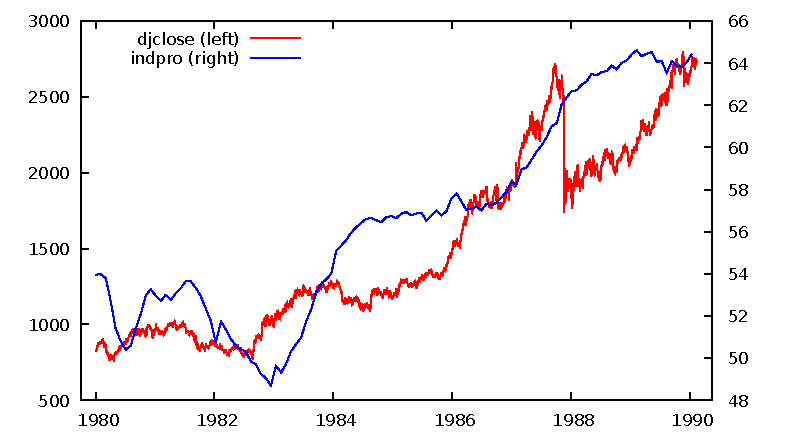
\includegraphics{figures/midas_daily_plot}
  \caption{Monthly industrial production and daily Dow Jones close}
  \label{fig:daily}
\end{figure}

\clearpage

\section*{Appendix C: parameterization functions}
\label{app:c}

Here we give some more detail of the MIDAS parameterizations supported
by gretl.

\vspace{1ex}

In general the normalized coefficient or weight $i$ ($i=1,\ldots,p$)
is given by
\begin{equation}
\label{eq:general}
  w_i = \frac{f(i,\theta)}
  {\sum_{k=1}^pf(k,\theta)}
\end{equation}
such that the coefficients sum to unity.

In the \textbf{normalized exponential Almon} case with $m$ parameters
the function $f(\cdot)$ is
\begin{equation}
f(i,\theta) = \exp\left(\sum_{j=1}^m \theta_j i^j\right)
\end{equation}
So in the usual two-parameter case we have
\[
w_i =
  \frac{\exp\left(\theta_1 i + \theta_2 i^2\right)}
  {\sum_{k=1}^p \exp\left(\theta_1 k + \theta_2 k^2\right)}
\]
and equal weighting is obtained when $\theta_1 = \theta_2 = 0$.

\vspace{1ex}

In the standard, two-parameter \textbf{normalized beta} case we have
\begin{equation}
\label{eq:fbeta}
  f(i, \theta) = (i^-/p^-)^{\theta_1-1} \cdot (1-i^-/p^-)^{\theta_2-1}
\end{equation}
where $p^- = p-1$, and $i^- = i-1$ except at the end-points, $i=1$ and
$i=p$, where we add and subtract, respectively, machine epsilon to
avoid numerical problems.  This formulation constrains the coefficient
on the last lag to be zero---provided that the weights are declining
at higher lags, a condition that is ensured if $\theta_2$ is greater
than $\theta_1$ by a sufficient margin. The special case of
$\theta_1 = \theta_2 = 1$ yields equal weights at all lags. A third
parameter can be used to allow a non-zero final weight, even in the
case of declining weights.  Let $w_i$ denote the normalized weight
obtained by using (\ref{eq:fbeta}) in (\ref{eq:general}). Then the
modified variant with additional parameter $\theta_3$ can be written
as
\[
w^{(3)}_i = \frac{w_i + \theta_3}{1 + p\theta_3}
\]
That is, we add $\theta_3$ to each weight then renormalize so that the
$w^{(3)}_i$ values again sum to unity.

In Eric Ghysels' Matlab code the two beta variants are labeled
``normalized beta density with a zero last lag'' and ``normalized beta
density with a non-zero last lag'' respectively.  Note that while the
two basic beta parameters must be positive, the third additive
parameter may be positive, negative or zero.

\vspace{1ex}

In the case of the plain \textbf{Almon polynomial} of order $m$,
coefficient $i$ is given by
\[
w_i = \sum_{j=1}^m \theta_j i^{j-1}
\]
Note that no normalization is applied in this case, so no additional
coefficient should be placed before the MIDAS lags term in the context
of a regression.

\subsection*{Analytical gradients}

Here we set out the expressions for the analytical gradients produced
by the \texttt{mgradient} function, and also used internally by the
\texttt{midasreg} command. In these expressions $f(i,\theta)$ should
be understood as referring back to the specific forms noted above
for the exponential Almon and beta distributions. The summation
$\sum_k$ should be understood as running from 1 to $p$.

For the normalized exponential Almon case, the gradient is
\begin{align*}
\frac{dw_i}{d\theta_j} &= 
\frac{f(i, \theta) i^j}{\sum_kf(k, \theta)} - 
\frac{f(i, \theta)}{\left[\sum_kf(k, \theta)\right]^2}
\, \sum_k\left[f(k, \theta) k^j\right] \\[4pt]
 &= w_i \left(i^j - 
\frac{\sum_k\left[f(k,\theta)k^j\right]}{\sum_k f(k, \theta)}\right)
\end{align*}

For the two-parameter normalized beta case it is
\begin{align*}
\frac{dw_i}{d\theta_1} &=
\frac{f(i,\theta) \log(i^-/p^-)}{\sum_k f(k, \theta)} -
\frac{f(i,\theta)}{\left[\sum_k f(k,\theta)\right]^2}
\sum_k\left[f(k,\theta) \log(k^-/p^-)\right] \\[4pt]
&= w_i \left(\log(i^-/p^-) - 
\frac{\sum_k\left[f(k,\theta) \log(k^-/p^-)\right]}{\sum_k 
 f(k,\theta)}\right) \\[8pt]
\frac{dw_i}{d\theta_2} &=
\frac{f(i,\theta) \log(1 - i^-/p^-)}{\sum_k f(k, \theta)} -
\frac{f(i,\theta)}{\left[\sum_k f(k,\theta)\right]^2}
\sum_k\left[f(k,\theta) \log(1 - k^-/p^-)\right] \\[4pt]
&= w_i \left(\log(1 - i^-/p^-) - 
\frac{\sum_k\left[f(k,\theta) \log(1 - k^-/p^-)\right]}{\sum_k 
 f(k,\theta)}\right)
\end{align*}

And for the three-parameter beta, we have
\begin{align*}
\frac{dw^{(3)}_i}{d\theta_1} &= 
  \frac{1}{1+p\theta_3} \, \frac{dw_i}{d\theta_1} \\
\frac{dw^{(3)}_i}{d\theta_2} &= 
  \frac{1}{1+p\theta_3} \, \frac{dw_i}{d\theta_2} \\
\frac{dw^{(3)}_i}{d\theta_3} &=
\frac{1}{1+p\theta_3} - \frac{p(w_i + \theta_3)}{(1+p\theta_3)^2}
\end{align*}

For the (non-normalized) Almon polynomial the gradient is simply
\[
\frac{dw_i}{d\theta_j} = i^{j-1}
\]

\end{document}
